\chapter{Конструкторский раздел}
\section{Диаграмма проектируемой базы данных}
На рисунке~\ref{fig:BD} представлена диаграмма  проектируемой базы данных.

\begin{figure}
	\centering
	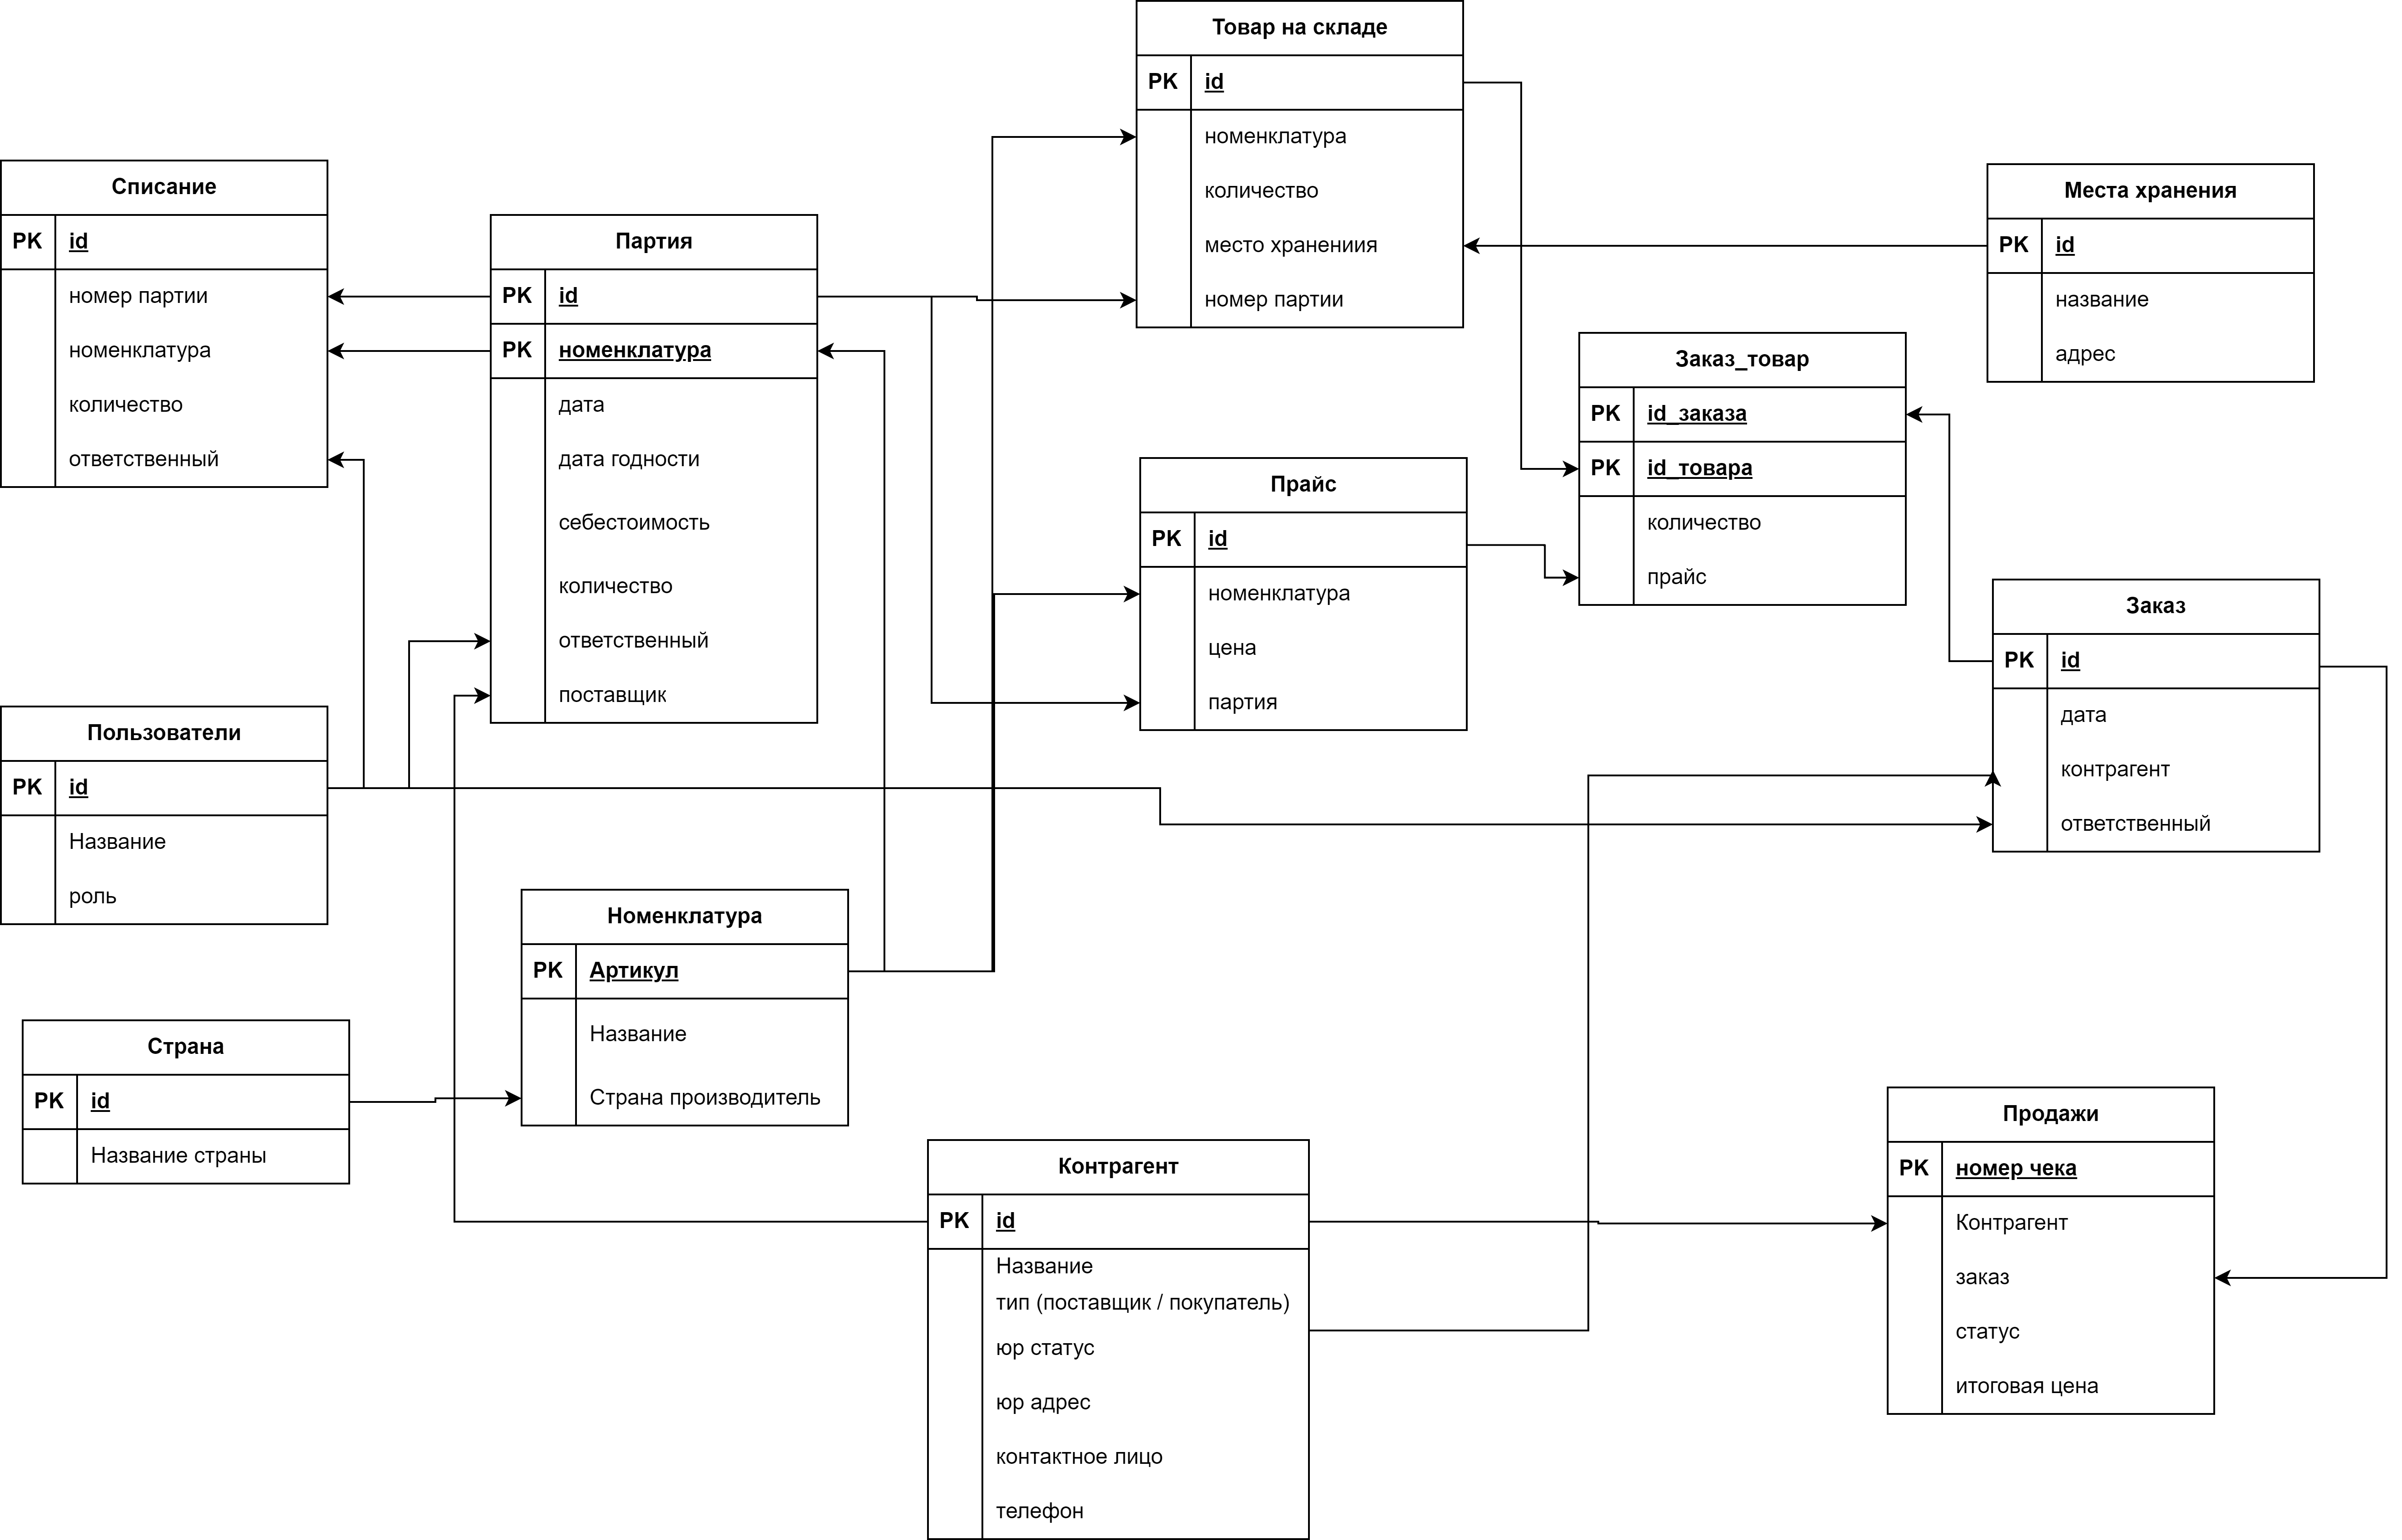
\includegraphics[width=1.5\linewidth, angle=-90]{pictures/BD_2}
	\caption{Диаграмма проектируемой базы данных}
	\label{fig:BD}
\end{figure}

\section{Описание сущностей проектируемой базы данных}
\begin{itemize}
	\item \textbf{Списание}
	\begin{itemize}
		\item Основная сущность для учёта списания товаров
		\item Атрибуты:
		\begin{itemize}
			\item id - уникальный идентификатор
			\item номер партии
			\item номенклатура
			\item количество списываемого товара
			\item ответственный за списание (пользователь с ролью кладовщик)
		\end{itemize}
	\end{itemize}
	
	\item \textbf{Пользователи}
	\begin{itemize}
		\item Сущность для хранения данных пользователей системы
		\item Атрибуты:
		\begin{itemize}
			\item id - уникальный идентификатор
			\item название (имя пользователя)
			\item роль в системе
		\end{itemize}
	\end{itemize}
	
	\item \textbf{Страна}
	\begin{itemize}
		\item Справочник стран
		\item Атрибуты:
		\begin{itemize}
			\item id - уникальный идентификатор
			\item название страны
		\end{itemize}
	\end{itemize}
	
	\item \textbf{Товар на складе}
	\begin{itemize}
		\item Сущность учёта текущих остатков на складе
		\item Атрибуты:
		\begin{itemize}
			\item id - уникальный идентификатор
			\item номенклатура
			\item количество товара
			\item место хранения
			\item номер партии
		\end{itemize}
	\end{itemize}
	
	\item \textbf{Заказ}
	\begin{itemize}
		\item Сущность для оформления заказов
		\item Атрибуты:
		\begin{itemize}
			\item id - уникальный идентификатор
			\item дата
			\item контрагент
			\item ответственный за заказ
		\end{itemize}
	\end{itemize}
	
	\item \textbf{Заказ товар}
	\begin{itemize}
		\item Сущность для сопоставления заказа и товаров
		\item Атрибуты:
		\begin{itemize}
			\item id заказа
			\item id товара
			\item количество
			\item прайс
		\end{itemize}
	\end{itemize}
	
	\item \textbf{Контрагент}
	\begin{itemize}
		\item Сущность для хранения данных контрагентов
		\item Атрибуты:
		\begin{itemize}
			\item id - уникальный идентификатор
			\item название
			\item тип (поставщик/покупатель)
			\item юридический статус
			\item юридический адрес
			\item контактное лицо
			\item телефон
		\end{itemize}
	\end{itemize}
	
	\item \textbf{Продажи}
	\begin{itemize}
		\item Сущность для учёта продаж
		\item Атрибуты:
		\begin{itemize}
			\item номер чека
			\item контрагент
			\item заказ
			\item статус продажи
			\item итоговая цена
		\end{itemize}
	\end{itemize}
	
	\item \textbf{Места хранения}
	\begin{itemize}
		\item Справочник складских помещений
		\item Атрибуты:
		\begin{itemize}
			\item id - уникальный идентификатор
			\item название места хранения
			\item адрес
		\end{itemize}
	\end{itemize}
	
	\item \textbf{Номенклатура}
	\begin{itemize}
		\item Основной справочник товаров/продукции
		\item Атрибуты:
		\begin{itemize}
			\item id - уникальный идентификатор
			\item название товара
			\item страна производства
		\end{itemize}
	\end{itemize}
	
	\item \textbf{Партия}
	\begin{itemize}
		\item Учёт поступлений товаров партиями
		\item Атрибуты:
		\begin{itemize}
			\item id - уникальный идентификатор
			\item дата
			\item дата годности
			\item себестоимость
			\item количество
			\item ответственный
			\item поставщик
		\end{itemize}
	\end{itemize}
	
	\item \textbf{Прайс}
	\begin{itemize}
		\item Справочник цен на товары
		\item Атрибуты:
		\begin{itemize}
			\item id - уникальный идентификатор
			\item номенклатура
			\item цена
			\item партия
		\end{itemize}
	\end{itemize}
	
\end{itemize}
\section{Описание проектируемых ограничений целостности базы данных}
\section{Описание всех проектируемых процедур/функций/триггеров в формате схемы}

\section{Описание проектируемой ролевой модели на уровне базы данных}
